\section{Proof Techniques for Conjunctive Systems} \label{gua:sec:proofs-conj}

\subsection{\LTLmX\ Properties Without Fairness: Existing Constructions} \label{gua:sec:ideas-conj-nofair}

The Monotonicity Lemma is proven~\cite{Emerson00} by keeping the additional process in the initial state.

\begin{lemma}[Monotonicity: Conj, \LTLmX, Unfair] \label{le:ConjMonotonicityLemma}
For conjunctive systems,
\begin{align*}
\forall n \geq 1:\ 
(A,B)^{(1,n)} \models \pexists h(A,B_1)
\ \ \Impl \ \ 
(A,B)^{(1,n+1)}\models \pexists h(A,B_1).
\end{align*}
\end{lemma}
\begin{proof}
Let the new process stutter in $\init$ state.
\end{proof}

To prove the Bounding Lemma,
Emerson and Kahlon \cite{Emerson00} suggest
to simply copy the local runs $x(A)$ and $x(B_1)$ into $y$. 
In addition,
we may need one more process that moves infinitely often
to ensure that an infinite run of \largesys will result in an infinite run of \cutoffsys.
All transitions of copied processes will be enabled
because removing processes from a conjunctive system
cannot disable a transition that was enabled before.

\begin{lemma}[Bounding: Conj, \LTLmX, Unfair] \label{le:ConjunctiveBoundingLemma}
For conjunctive systems,
\begin{align*}
\forall n \geq 2:\ 
(A,B)^{(1,2)} \models \pexists h(A,B_1)
\ \ \Implied \ \ 
\largesys \models \pexists h(A,B_1).
\end{align*}
\end{lemma}
The proof is inspired by the first part of the proof of \cite[Lemma 5.2]{Emerson00}.
\begin{proof}
Let $x=(s_1,e_1,p_1) (s_2,e_2,p_2) \ldots$ be a run of $\largesys$. 
Note that, by the semantics of conjunctive guards, 
the transitions along any local run of $x$ will also be enabled 
in any system $\cutoffsys$ with $c \leq n$, 
where the processes exhibit a subset of the local runs of $x$. 
Thus, we obtain a run of $\cutoffsys$ by copying a subset of the local runs of $x$, 
and removing elements of the new global run where all processes stutter.
\sj{should we put this as a general lemma somewhere?}

Then, based on an infinite run $x$ of the original system, 
we construct an infinite run $y$ of the cutoff system. 
Let $y(A)=x(A)$ and $y(B_1)=x(B_1)$. 
The second copy of template $B$ in $(A,B)^{(1,2)}$ is needed to ensure that 
the run $y$ is infinite, i.e., at least one process moves infinitely often. 
If both $x(A)$ and $x(B_1)$ eventually deadlock, 
then there exists a process $B_i$ of $\largesys$ that makes infinitely many moves, 
and we set $y(B_2) = x(B_i)$. 
Otherwise, we set $y(B_2) = x(B_2)$.
\end{proof}

\begin{tightness}[Conj, \LTLmX, Unfair] \label{obs:conj:tight_prop}
The cutoff $c=2$ is tight for parameterized model checking of properties $\pexists h(A,B_1)$ in the 1-conjunctive systems, i.e., there is a system type $(A,B)$ and property $Eh(A,B_1)$ which is not satisfied by $(A,B)^{(1,1)}$ but is by $(A,B)^{(1,2)}$.
\end{tightness}
\begin{proof}
Figure~\ref{fig:obs:conj:tight_prop} shows templates $(A,B)$, $\pexists h(A,B_1) = \pexists \eventually b$. An infinite run that satisfies the formula needs one copy of $B$ that stays in the initial state, and one that moves into $b$.
\begin{figure}[tb]
\centering
\begin{subfigure}[b]{0.45\textwidth}\center
\scalebox{0.75}{% !TEX root = table.tex
\begin{tikzpicture}[node distance=1.5cm,inner sep=1pt,minimum size=0.5mm,->,>=latex]


\node[state,initial left] (init) {};
\path (init) [loop right] edge [right] node {$\forall \neg 1_B$} (init);



\end{tikzpicture}
  }
\caption*{Template A}
\end{subfigure}
\begin{subfigure}[b]{0.45\textwidth}\center
\centering
\scalebox{0.75}{% !TEX root = table.tex
\begin{tikzpicture}[node distance=1.5cm,inner sep=1pt,minimum size=0.5mm,->,>=latex]


\node[state,initial left] (init) {};
\node[state] (b_1) [right= of init] {$1_B$};

\path (init) edge [above] node {} (b_1);
\path (init) [loop below] edge [right] node {} (init);


\end{tikzpicture}
  
}
\caption*{Template B}
\end{subfigure}
\caption{Templates used to prove Tightness~\ref{obs:conj:tight_prop}}
\label{fig:obs:conj:tight_prop}
\end{figure}
\end{proof}


\subsection{\LTLmX\ Properties with Fairness: New Constructions} \label{gua:sec:ideas-conj-fair}

In this section, subscript $i$ in path quantifiers, $\pexists_i$ and $\pforall_i$, 
denotes the quantification over initializing runs.

The proof of the Bounding Lemma is the same as in the non-fair case,
noting that, if the original run is unconditional-fair,
then so will be the resulting run.

\begin{lemma}[Bounding: Conj, \LTLmX, Fair] \label{le:FairConjunctiveBounding Lemma}
For unconditionally-fair initializing runs of conjunctive systems:
\begin{align*}
&\forall n \geq 1:\\
& (A,B)^{(1,1)} \models \pexists_{uncond} h(A,B_1)
\ \Implied \
(A,B)^{(1,n)} \models \pexists_{uncond} h(A,B_1).
\end{align*}
\end{lemma}
\begin{proof}
Given an unconditionally-fair [initializing] run $x$ of $\largesys$ with $n>c$ construct an unconditionally-fair [initializing] run $y$ in the cutoff system $(A,B)^{(1,1)}$: copy the local runs of processes $A$, $B_1$.
%  and copy the behaviour of a process of $\largesys$ that moves infinitely often in the run $x$. Since $y$ is the result of removal of a number of local runs from $x$, it is an unconditionally-fair initializing run of $\cutoffsys$.
\end{proof}

Proving the Monotonicity Lemma is more difficult,
since the fair extension construction from disjunctive 
systems does not work for conjunctive systems%
---if an additional process mimics the transitions of an existing process
   then it disables transitions of the form 
   $\transition{q}{q'}{\textit{``\,}\forall\neg q\textit{\!''}}$ or
   $\transition{q}{q'}{\textit{``\,}\forall\neg q'\textit{\!''}}$.
Hence, we add the restriction of initializing runs, 
which allows us to construct a fair run as follows.
The additional process $B_{n+1}$ ``shares'' a local run $x(B_i)$ 
with an existing process $B_i$ of $(A,B)^{(1,n+1)}$: 
one process stutters in $\init_B$ while the other makes transitions from $x(B_i)$, 
and whenever $x(B_i)$ enters $\init_B$
(this happens infinitely often),
the roles are reversed. 
Since this changes the behavior of $B_i$, 
$B_i$ should not be mentioned in the formula, 
i.e., we need $n\geq 2$ for a formula $h(A,B^{(1)})$. 

\begin{lemma}[Monotonicity: Conj, \LTLmX, Fair] \label{le:ConjMonFair}
For unconditionally-fair initializing runs of conjunctive systems:\sj{generalization is obvious; $n \ge k+1$ in general case}
\begin{align*}
& \forall n \ge 2:\\
& (A,B)^{(1,n)} \models \pexists_{uncond,i} h(A,B_1)
\ \Impl \
(A,B)^{(1,n+1)} \models \pexists_{uncond,i} h(A,B_1).
\end{align*}
\end{lemma}
\begin{proof}
Given a unconditionally-fair initializing run $x$ of $\largesys$, we construct a unconditionally-fair initializing run $y$ in $(A,B)^{(1,n+1)}$, with one additional process $p$. 
First, copy all local runs of all processes of $(A,B)^{(1,n)}$ from the run $x$ into $y$.
Then, let process $p'$ stutter in $\init$ until some other process $p \neq B_1$ enters $\initstate$. 
Then, exchange the roles of processes $p'$ and $p$: let $p$ stutter in $\initstate$, while $p'$ takes the transitions of $p$ from the original run, until it enters $\initstate$. And so on.
In this way, we continue to interleave the run between $p'$ and $p$, and obtain a unconditionally-fair initializing run for all processes, with $y(A,B_1)=x(A,B_1)$. 
Thus, if $\largesys \models \pexists h(A,B_1)$, then $(A,B)^{(1,n+1)} \models \pexists h(A,B_1)$.
\end{proof}


\begin{tightness}[1-Conj, \LTLmX, Fair] \label{obs:conj:tight_prop_fair}
The cutoff $c=2$ is tight for parameterized model checking of $\pexists h(A,B_1)$ 
on unconditionally-fair initializing runs in 1-conjunctive systems, 
i.e., 
there is a system type $(A,B)$ and property $\pexists h(A,B_1)$ 
which is satisfied by $(A,B)^{(1,1)}$ but not by $(A,B)^{(1,2)}$.
\end{tightness}
\begin{proof}
Figure~\ref{fig:obs:conj:tight_prop_fair} shows templates $(A,B)$;
$\pexists h(A,B_1) = \pexists \FG (b_{init} \impl a_1)$.
\begin{figure}[tb]
\centering
\begin{subfigure}[b]{0.45\textwidth}\center
\scalebox{0.75}{% !TEX root = table.tex
\begin{tikzpicture}[node distance=1.5cm,inner sep=1pt,minimum size=0.5mm,->,>=latex]


\node[state,initial left] (init) {${init}_A$};
\node[state] (a_1) [right= of init] {$1_A$};

\path (init) edge [above] node {} (a_1);
\path (a_1)  [bend left=20] edge [below] node {} (init);



\end{tikzpicture}
  }
\caption*{Template A}
\end{subfigure}
\begin{subfigure}[b]{0.45\textwidth}\center
\scalebox{0.75}{% !TEX root = table.tex
\begin{tikzpicture}[node distance=1.5cm,inner sep=1pt,minimum size=0.5mm,->,>=latex]


\node[state,initial left] (init) {${init}_B$};
\node[state] (b_1) [right= of init] {$1_B$};
\node[state] (b_2) [right= of b_1] {$2_B$}; 

\path (init) edge [above] node {$\forall\neg 1_B$} (b_1);
\path (b_1)  edge [above] node {$\forall\neg 1_A$} (b_2);
\path (b_2)  [bend left=20] edge [below] node {$\forall\neg 2_B$} (init);



\end{tikzpicture}
  
}
\caption*{Template B}
\end{subfigure}
\caption{Templates used to prove Tightness~\ref{obs:conj:tight_prop_fair}}
\label{fig:obs:conj:tight_prop_fair}
\end{figure}
\end{proof}


\subsection{Deadlocks Without Fairness: Updated Constructions}\label{gua:sec:proofs-conj-deadlock-unfair}

\begin{lemma}[Monotonicity: Conj, Deadlocks, Unfair] \label{le:ConjunctiveMonotonicityLemmaDeadlocks}
For conjunctive systems:
$$
\forall n\geq 1: (A,B)^{(1,n)} \textit{ has a deadlock} 
\ \Impl\ 
(A,B)^{(1,n+1)} \textit{ has a deadlock.}
$$
\end{lemma}
\begin{proof}
Given a deadlocked run $x$ of $(A,B)^{(1,n)}$, we construct a deadlocked run of $(A,B)^{(1,n+1)}$.
Let $y$ copy run $x$, and keep the new process in $\init$.
If $x$ is globally deadlocked and $d$ is the moment when the deadlock happens in $x$,
then schedule the new process arbitrarily after moment $d$.
Thus, it is possible that the newly constructed system run is only locally deadlocked,
while the original run is globally deadlocked.
\end{proof}


As for the Bounding Lemma,
in the case of global deadlock detection, 
Emerson and Kahlon~\cite{Emerson00} suggest to copy a subset of the original local runs.
For every local state $q$ that is present in the final state of the run, 
we need at most two local runs that end in this state. 
In the case of local deadlocks, 
our construction uses the fact that systems are 1-conjunctive.
In 1-conjunctive systems, if a process is deadlocked, 
then there is a set of states $DeadGuards$ that all need to be populated by other processes
in order to disable all transitions of the deadlocked process. 
Thus, the construction copies: 
(i) the local run of a deadlocked process, 
(ii) for each $q \in DeadGuards$, the local run of a process 
     that is in $q$ at the moment of the deadlock, and
(iii) the local run of an infinitely moving process.

\begin{lemma}[Bounding: 1-Conj, Deadlocks, Unfair] \label{le:ConjunctiveBoundingLemmaDeadlocks}
For 1-conjunctive systems:
\li
  \- with $c=2|Q_B\smi \{ \init \}|$ and any $n>c$ \footnote{This statement also applies to systems without restriction to $1$-conjunctive guards.}
  $$(A,B)^{(1,c)} \textit{ has a global deadlock} \ \Implied\ (A,B)^{(1,n)} \textit{ has a global deadlock;} $$
  
  \- with $c=|Q_B\smi \{ \init \}|+2$ and any $n>c$:
  $$(A,B)^{(1,c)} \textit{ has a local deadlock} \ \Implied\ (A,B)^{(1,n)} \textit{ has a local deadlock;}$$
  
  \- with $c=2|Q_B\smi \{ \init \}|$ and any $n>c$:
  $$(A,B)^{(1,c)} \textit{ has a deadlock} \ \Implied\ (A,B)^{(1,n)} \textit{ has a deadlock.}$$
\il
\end{lemma}
\begin{proof}
The proof is inspired by the second part of the proof of \cite[Lemma 5.2]{Emerson00}, 
but in addition to global we consider local deadlocks. 

\myparagraph{Global deadlocks} 
Let $c=2|Q_B\smi\{ \init \}|)$. 
Let run $x = (s_1,e_1,p_1)\ldots(s_d,e_d,\bot)$ of \largesys 
with $n>c$ be globally deadlocked. 
We construct a globally deadlocked run $y$ in $\cutoffsys$ as follows.
\li
  \-[a.] For every $q \in s_d \setminus \{\init\}$:
  \li
    \- if $s_d$ has two processes in state $q$, 
       then devote two processes of \cutoffsys that mimic the behaviour 
       of the two of \largesys correspondingly;

    \- otherwise, $s_d$ has only one process in state $q$, 
       then devote one process of \cutoffsys that mimics the process of \largesys;
  \il
  \-[b.] for every process of \cutoffsys not used in the construction (if any): 
         let it mimic an arbitrary $B$-process of \largesys
         that was not yet used in the construction in item (a) nor (b).
\il
The construction uses $\leq 2|Q_B\smi \{ \init \}|$ processes $B$.
Note that the proof does not assume that the system is 1-conjunctive.

\myparagraph{Local deadlocks} 
Let $c = |Q_B\smi \{ \init \}|+2$. 
Let run $x = (s_1,e_1,p_1)\ldots$ of \largesys with $n>c$ be locally deadlocked. 
We will construct a run $y$ of \cutoffsys 
where at least one process deadlocks and exactly one process moves infinitely often.

Wlog. we distinguish three cases:
\li
\-[1.] $A$ moves infinitely often in $x$, and $B_1$ deadlocks;
\-[2.] $A$ deadlocks, and $B_1$ moves infinitely often; and
\-[3.] $A$ neither deadlocks nor moves infinitely often, $B_1$ deadlocks, 
       $B_2$ moves infinitely often.
\il

\myparagraph{1} ``$A$ moves infinitely often in $x$, and $B_1$ deadlocks''.

Let $q_\bot, e_\bot$ be the deadlocked state and input of $B_1$ in $x$, 
and let $d$ be the moment from which $B_1$ is deadlocked.

Let $DeadGuards=\{q_1,\ldots,q_k\}$ be the set of states
such that for every $q_i \in DeadGuards$ there is an outgoing transitions 
from $q_\bot$ with $e_\bot$ guarded ``$\forall \neg q_i$'',
and assume $DeadGuards \neq \emptyset$
(if it is empty, then we keep every process in $\init$ 
 until someone reaches $q_\bot$ and then schedule the rest arbitrarily). 
(Recall that $q_i \in Q_B \cupdot Q_A$.)

The construction is as follows.
\li
  \-[a.] $y(A)=x(A)$, $y(B_1)=x(B_1)$.
  \-[b.] For each $q \in DeadGuards$, at moment $d$ in $x$
         there is a process $p_q$ in state $q$. 
         If $p_q \in \{B_1,...,B_n\}$, 
         then let one process of \cutoffsys mimic it till moment $d$, 
         and then stutter in $q$.
  \-[c.] Let other processes of \cutoffsys (if any) stay in $\init$.
\il
The construction uses (if ignore (c)) $\leq |Q_B\smi \{ \init \}|+1$ processes $B$.

Note: 
the assumption of 1-conjunctive systems implies that,
in order to deadlock $B_1$,
we need a process in each state in $BlockGuards$.
This implies that having a process in each state of $BlockGuards$ does not disable 
any $A$'s transition after moment $d$.

\myparagraph{2} ``$A$ deadlocks, and $B_1$ moves infinitely often'': 
use the construction from (1).

\myparagraph{3} 
``$A$ neither deadlocks nor moves infinitely often, 
  $B_1$ deadlocks, $B_2$ moves infinitely often''. 
Use the construction from (1), and additionally: $y(B_2)=x(B_2)$. 
Thus, the construction uses (if ignore (c)) $\leq |Q_B \smi \{ \init \}|+2$ 
processes $B$.

\myparagraph{Deadlocks}
Take the higher value among the cases considered above $c=2|Q_B\smi \{ \init \}|$: 
if $x$ is locally deadlocked then the Monotonicity Lemma ensures 
that there is a deadlocked run in \cutoffsys.
\end{proof}


\begin{tightness}[1-Conj, Deadlocks, Unfair] \label{obs:conj:tight_deadlock}
The cutoff $c=2|B|-2$ is tight for parameterized deadlock detection in the 1-conjunctive systems, i.e., for any $k$ there is a system type $(A,B)$ with $|B|=k$ such that there is a deadlock in $(A,B)^{(1,2|B|-2)}$, but not in $(A,B)^{(1,2|B|-3)}$. 
\end{tightness}
\begin{proof} 
Figure~\ref{fig:obs:conj:tight_deadlock} provides templates $(A,B)$ that proves the observation. In the figure the edge with $\forall{\neg b_1},\ldots,\forall{\neg b_k}$ denotes edges with guards $\forall{\neg b_1},\ldots,\forall{\neg b_k}$. To get the global deadlock we need at least two processes in each $b_i \in \{b_1,\ldots,b_k\}$. Note that the system does not have local deadlocks.\ak{show that cutoffs for local deadlocks are also tight}
\begin{figure}[h]
\vspace{-10pt}
\centering
\begin{subfigure}[b]{0.45\textwidth}\center
\scalebox{0.75}{% !TEX root = table.tex
\begin{tikzpicture}[node distance=2.3cm,inner sep=1pt,minimum size=0.5mm,->,>=latex]


\node[initial left, state] (init) {};

\path (init) [loop right] edge [right] node {$\forall\neg 1_B$} (init);
\path (init) [loop right,dotted,distance=26mm] edge [right] node {...} (init);
\path (init) [loop right,distance=38mm] edge [right] node {$\forall\neg k_B$} (init);


\end{tikzpicture}
  
}
\caption*{Template A}
\end{subfigure}
\hspace{1cm}
\begin{subfigure}[b]{0.45\textwidth}\center
\scalebox{0.75}{% !TEX root = table.tex
\begin{tikzpicture}[node distance=2.4cm,inner sep=1pt,minimum size=0.5mm,->,>=latex]


\node[initial above, state] (init) {$init$};
\node[state] (b_1) [left=2.7cm of init] {$1_B$};
\node (dots) [below=1cm of init] {$\ldots$};
\node[state] (b_k) [right=2.7cm of init] {$k_B$}; 

% \path (b_1.20) edge [above] node {\specialcell{$\forall{\neg b_1}$\\...\\$\forall{\neg b_k}$}} (init.160);
\path (b_1.20) edge [above] node {$\forall{\neg 1_B},...,\forall{\neg k_B}$} (init.160);
\path (init.200) edge [above] node {} (b_1.340);

\path (b_k.160) edge [above] node {$\forall{\neg 1_B},...,\forall{\neg k_B}$} (init.20); 
\path (init.340) edge [above] node {} (b_k.200); 

\path (init.282) edge [left, dotted] node {} ($(dots)+(0.1,0.1)$);
\path ($(dots)-(0.1,-0.1)$) edge [left, dotted] node {$\forall{\neg 1_B},...,\forall{\neg k_B}$} (init.257);

% \path (b_1) [loop left] edge [left] node {$\forall\neg b_1$} (b_1);
% \path (b_1) [loop left,dotted,distance=26mm] edge [left] node {...} (b_1);
% \path (b_1) [loop left,distance=38mm] edge [left] node {$\forall\neg b_k$} (b_1);

% \path (b_k) [loop right] edge [right] node {$\forall\neg b_1$} (b_k);
% \path (b_k) [loop right,dotted,distance=26mm] edge [right] node {...} (b_k);
% \path (b_k) [loop right,distance=38mm] edge [right] node {$\forall\neg b_k$} (b_k);


\end{tikzpicture}
  
}
\caption*{Template B}
\end{subfigure}
\caption{Templates used to prove Tightness~\ref{obs:conj:tight_deadlock}}
\label{fig:obs:conj:tight_deadlock}
\end{figure}
\end{proof}


\subsection{Deadlocks with Fairness: New Constructions} \label{gua:sec:proofs-conj-deadlock-fair}

The Monotonicity Lemma is proven by keeping process $B_{n+1}$ in the initial state, 
and copying the runs of deadlocked processes.
If the run of \largesys is globally deadlocked,
then process $B_{n+1}$ may keep moving in the constructed run,
i.e., the run may be only locally deadlocked. 
In the case of a local deadlock in \largesys, we distinguish two cases: 
there is an infinitely moving $B$-process, or all $B$-processes are deadlocked 
(and thus $A$ moves infinitely often).
In the latter case, we use the same construction as in the global deadlock case
(the correctness argument uses the fact that systems are 1-conjunctive, 
 runs are initializing, and there is only one process of type $A$).
In the former case, we copy the original run, and let $B_{n+1}$ share
a local run with an infinitely moving $B$-process.

\begin{lemma}[Monotonicity: Conj, Deadlocks, Fair] \label{le:FairConjunctiveMonotonicityLemmaDeadlocks}
For 1-conjunctive systems on strong fair initializing or finite runs:
$$
\forall n\geq 1: (A,B)^{(1,n)} \textit{ has a deadlock}
\ \Impl\ 
(A,B)^{(1,n+1)} \textit{ has a deadlock.}
$$
\end{lemma}
\begin{proof}\ak{check the minimal value of $n$ (1 or 2?)}
Let $x$ be a globally deadlocked or locally deadlocked strong-fair initializing run of $(A,B)^{(1,n)}$.
We will build a globally deadlocked or locally deadlocked strong-fair initializing run 
of $(A,B)^{(1,n+1)}$.

If $x$ is finite, then $y$ is the copy of $x$, and the new process stays in $\init_B$
until every process becomes deadlocked, and then is scheduled arbitrarily.
Note that $y$ constructed this way may be locally deadlocked 
rather than globally deadlocked as $x$ is.

Now consider the case when $x$ is locally deadlocked strong-fair initializing.

Let $\mD$ be the set of deadlocked $B$-processes in $x$, and $d$ be the moment 
when the processes become deadlocked.

Consider the case $\visInf{\mB\smi\mD}{x} \neq \emptyset$:
copy $x$ into $y$, and let the new process $B_{n+1}$ wait in $\init_B$ 
and interleave the roles with a process $B$ that moves infinitely often in $x$, 
as described in the proof of Lemma~\ref{le:ConjMonFair}.

Consider the case $\visInf{\mB\smi\mD}{x} = \emptyset$:
every $B$ process of $(A,B)^{(1,n)}$ is deadlocked and thus $\mD = \mB$.
Define 
$$
DeadGuards\! =\! \big\{q \| \exists B_i \in \mD
                      \textit{ with a transition guarded ``\,}
                      {\forall \neg q} 
                      \textit{\!'' in } (s_d(B_i),e_d(B_i))\big\}.
$$
Note that $Q_A \cap DeadGuards = \emptyset$, because $A$ visits infinitely often $\init_A$
and we consider 1-conjunctive systems.
Hence, copy $x$ into $y$, and let the new process $B_{n+1}$ wait in $\init_B$ 
until every process $B_1,...,B_n$ become deadlocked, and then schedule $B_{n+1}$ arbitrarily.
%
% See the proof of Lemma~\ref{le:ConjunctiveMonotonicityLemmaDeadlocks}.
%%% AK: this won't work because the process B_{n+1} in init should move inf often or deadlock,
%%% the arbitrary scheduling can lead to unlocking of every one
\end{proof}


As for the Bounding Lemma,
we use a construction that is similar to that of properties under fairness for disjunctive systems (Sect.~\ref{gua:sec:ideas-disj-fair}):
  in the setup phase, 
  we populate some ``safe'' set of states with processes,
  and then we extend the runs of non-deadlocked processes 
  to satisfy strong fairness, 
  while ensuring that deadlocked processes never get enabled.

\begin{lemma}[Bounding: 1-Conj, Deadlocks, Fair] \label{le:FairConjunctiveBoundingLemmaDeadlocks}
For 1-conjunctive systems on strong-fair initializing or finite runs:
\ak{no real need for initializing -- but easier to explain}
\li
  \- with $c=2|Q_B\smi \{ \init \}|$ and any $n>c$:
  $$
  \cutoffsys \textit{ has a global deadlock} 
  \ \Implied\ 
  \largesys \textit{ has a global deadlock;}
  $$

  \- with $c=2|Q_B\smi \{ \init \}|+1$ and any $n>c$ (when $|Q_B|>2$):
  $$
  \cutoffsys \textit{ has a local deadlock} 
  \ \Implied\ 
  \largesys \textit{ has a local deadlock;}
  $$

  \- with $c=2|Q_B\smi \{ \init \}|$ and any $n>c$:
  $$
  \cutoffsys \textit{ has a deadlock} 
  \ \Implied\ 
  \largesys \textit{ has a deadlock.}
  $$
\il
\end{lemma}
\begin{proof}
\providecommand{\deadOne}{\dead_1}
\providecommand{\deadTwo}{\dead_2}

\myparagraph{Global deadlocks}
$c=2|Q_B \smi \{\init_B\}|$, 
see Lemma~\ref{le:ConjunctiveBoundingLemmaDeadlocks}, 
the fairness does not matter on finite runs.

\myparagraph{Local deadlocks}
Let $c=2|Q_B\smi \{ \init_B \}|$. 
Let $x= (s_1,e_1,p_1)\ldots$ be a locally deadlocked strong-fair intitializing run 
of $\largesys$ with $n>c$. 
We construct a locally deadlocked strong-fair initializing run $y$ of $\cutoffsys$.

Let $\mD$ be the set of deadlocked processes in $x$. 
Let $d$ be the moment in $x$ starting from which every process in $\mD$ is deadlocked.

Let $\dead(x)$ be the set of states in which processes $\mD$ of \largesys
are deadlocked.

Let $\deadTwo(x) \subseteq \dead(x)$ be the set of deadlocked states such that: 
for every $q \in \deadTwo(x)$, 
there is a process $P \in \mD$ with $s_d(P) = q$ 
and that for input $e_{\geq d}(P)$ has a transition guarded with ``$\forall \neg q$''.
Thus, a process in $q$ is deadlocked with $e_d(P)$
only if there is another process in $q$ in every moment $\geq d$.

Let $\deadOne(x) = \dead(x)\smi\deadTwo(x)$.
I.e., 
for any $q \in \deadOne(x)$, there is a process $P$ of \largesys 
which is deadlocked in $s_d(P) = q$ with input $e_d(P)$,
and no transitions from $q$ with input $e_d(P)$ are guarded with ``$\forall \neg q$''.
%%% AK:
%%% Note that this def of deadOne differs from the below one (that i used originally):
%%% for every $q \in \deadOne(x)$, 
%%% there is a process $P \in \mD$ of \largesys
%%% that for input $e_{\geq d}(P)$ does not have a transition guarded with ``$\forall \neg q$''.
%%% The definition currently used may define deadOne which has less states that the commented one.
%%% But in the commented version we used the trick "Wlog., assume deadOne \cap deadTwo = 0", 
%%% which seems to produce the same set of states!

%Similarly, let $\deadOne(x)$ be the set of deadlocked states such that: 
%for every $q \in \deadOne(x)$, 
%there is a process $P \in \mD$ of \largesys
%that for input $e_{\geq d}(P)$ does not have a transition guarded with ``$\forall \neg q$''.
%I.e., 
%for such process $P$ is deadlocked in $q \in \deadOne(x)$ with input $e_{\geq d}(P)$,
%even if there is no other process in $q$ at any moment after $d$.
%
%Wlog., assume that $\deadOne(x) \cap \deadTwo(x) = \emptyset$.
%\footnote{Note:
%it is possible that
%$\deadOne \cap \deadTwo \neq \emptyset$ 
%for some locally deadlocked strong-fair initializing run $x$.
%But from $x$ we can always produce a locally deadlocked strong-fair initializing
%run $x'$ with an empty intersection as follows.
%Let $q \in \deadOne \cap \deadTwo$.
%Then, there is a process, $p \in {B_1,...,B_n}$, 
%deadlocked in $q$ with input $e(p)$ such that 
%all outgoing transitions from $q$ with $e(p)$ are not guarded with 
%``$\forall \neg q$''.
%Then, to all processes deadlocked in $q$ we provide input $e(p)$.
%This removes state $q$ from $\deadTwo$.
%By modifying inputs to all processes deadlocked in a state in the intersection,
%we can produce $x'$ with the empty intersection.
%}

%Let $\visited^\inf(x)$ be the set of states that are entered and
%exited infinitely often in $x$
%(this definition is slightly different from that of the rest of the paper).

%\ak{redefine the previous $\visited^\inf$ to mean: ``entered and exited inf often''?}

%Note:
%it is possible that $\dead(x) \cap \visited^\inf(x) \neq \emptyset$:
%one process may be deadlocked in such state provided one input,
%while another process may enter and exit the state infinitely often
%provided a different input.
% we cannot deadlock those non-deadlocked processes that
% visit $dead$, 
% because they might be moving on the loop that deadlocks some states,
% and deadlocking this process would require to move others from their states
% and BOOM! everyone gets unlocked!

Define
$$
DeadGuards\!=\!
\big\{ q \| \exists B_i \in \mD
         \textit{ with a transition guarded ``\,}
         {\forall \neg q} 
         \textit{\!'' in } (s_d(B_i),e_d(B_i)) \big\}.
$$
Figure~\ref{fig:conj-deadlocks-venn} illustrates properties of sets 
$DeadGuards$, $\deadOne$, $\deadTwo$, $\visInf{\mB\smi\mD}{x}$.
\ak{check how $A$'s states affect all those sets, currently i assumed that they are all subsets of $Q_B$}

\begin{figure}[hptb]
\begin{mdframed}
\centering
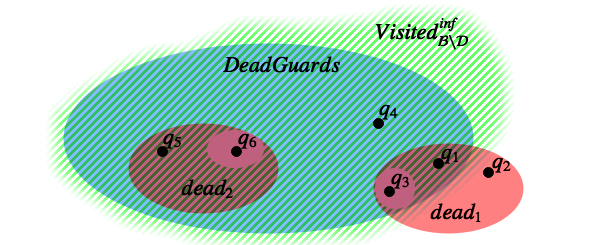
\includegraphics[width=0.7\textwidth]{guarded-systems/img/conj-deadlocks-venn.png}
\captionsetup{singlelinecheck=off}
\caption[fig:conj-deadlocks-venn]{%
Venn diagram for sets $DeadGuards$, $\deadOne$, $\deadTwo$, $\visInf{\mB\smi\mD}{x}$:
\begin{itemize}
\item[($q_1$)] $\deadOne \cap DeadGuards \cap \visInf{\mB\smi\mD}{x} \neq \emptyset$ is possible:
               in $x$, 
               there is a process deadlocked in state $q_1$,
               there is a non-deadlocked process that visits $q_1$ infinitely often,
               and there is a process deadlocked in a state $q \neq q_1$ 
               with a transition guarded ``$\forall \neg q_1$'' 

\item[($q_3$)] $\deadOne \cap DeadGuards \smi \visInf{\mB\smi\mD}{x} \neq \emptyset$ is possible:
               similarly to $q_1$, 
               except that no non-deadlocked processes visit $q_3$ infinitely often

\item[($q_2$)] $\deadOne \smi (\visInf{\mB\smi\mD}{x} \cup DeadGuards) \neq \emptyset$ is possible:
               in $x$, 
               there is a process deadlocked in state $q_2$,
               no other processes visit $q_2$ infinitely often,
               and no processes are deadlocked with a transition guarded ``$\forall \neg q_2$''

\item[($q_4$)] $DeadGuards \smi \dead \neq \emptyset$ is possible:
               there is a process deadlocked in a state $q \neq q_4$ 
               with a transition guarded  ``$\forall \neg q_4$''

\item[($q_5$)] $\deadTwo \cap \visInf{\mB\smi\mD}{x} \cap DeadGuards \neq \emptyset$ is possible:
               there is at least one process deadlocked in $q_5$ with a transition guarded ``$\forall \neg q_5$'',
               and some non-deadlocked process visits $q_5$ infinitely often
               (this process does not deadlock in $q_5$, 
                because in $q_5$ it receives an input different from that of the deadlocked processes)

\item[($q_6$)] $\deadTwo \cap DeadGuards \smi \visInf{\mB\smi\mD}{x} \neq \emptyset$ is possible:
               similarly to $q_5$, except no non-deadlocked processes visit $q_6$ infinitely often
\end{itemize}
}
\label{fig:conj-deadlocks-venn}
\end{mdframed}
\end{figure}

Let us assume $DeadGuards \neq \emptyset$---the other case is straightforward.\ak{check}

The construction has two phases, the setup and the looping phase.

In the {\bf setup phase}, we copy from $x$ into $y$:
\li
\-[a.] $y(A) = x(A)$;

\-[b.] for every $q \in \deadOne$: 
   devote one process of \cutoffsys that copies 
   a process of \largesys deadlocked in $q$;

\-[c.] for every $q \in \deadTwo \setminus \visInf{\mB\smi\mD}{x}$: 
   devote two processes of \cutoffsys that copy 
   the behaviour of two processes of \largesys that deadlock in $q$;

\-[d.] for every $q \in \deadTwo \cap \visInf{\mB\smi\mD}{x}$:
   in $x$, 
   there is a process, $B_q^\inf \in \mB\smi\mD$, that visits $q$ infinitely often,
   and there is a process, $B_q^\bot \in \deadTwo$, deadlocked in $q$.
   Then:
\li
   \-[1.] devote one process of \cutoffsys that copies the behaviour of $B_q^\bot$, and
   \-[2.] devote one process of \cutoffsys that copies the behaviour of $B_q^\inf$ 
          until it reaches $q$ at a moment after $d$,
          and then provide the same input as $B_q^\bot$ receives at moment $d$.
          This will deadlock the process;
\il

\-[e.] for every $q \in DeadGuards \setminus \dead$:
       note that $q \in \visInf{\mB\smi\mD}{x}$ and, thus, there is a process, 
       $B_q^\inf \in \mB\smi\mD$, 
       that visits $q$ infinitely often.
       Devote one process of \cutoffsys that copies the behaviour of $B_q^\inf$ 
       until it reaches $q$ at a moment after $d$;

\-[f.] if $DeadGuards \setminus \dead \neq \emptyset$ 
       or $A \in \mD$,
       then devote one process that stays in $\init_B$.
       The process will be used in the looping phase to ensure that the run $y$ is infinite,
       and that every process of \cutoffsys used in (e) 
       moves infinitely often (and thus $y$ is strong-fair);
       and
%       Note that if $A$ moves infinitely often in $x$ and $DeadGuards \smi \dead = \emptyset$,
%       then there is no need for such additional infinitely moving process.

\-[g.] let any other process of \cutoffsys (if any) 
       copy behaviour of a process of \largesys 
       that was not used in the construction so far (including this step).
\il
\ak{go through every item, and prove it is necessary (by giving an example)}
The setup phase ensures: 
in every state $q \in \dead$,
there is at least one process deadlocked in $q$ at moment $d$ in $y$. 
Now we need to ensure that the non-deadlocked processes described 
in steps (e) and (f) move infinitely often,
which is done using the looping extension described bellow.

The looping phase is applied to processes in (e) and (f) only\footnote%
{%
  If there are no such processes, then the setup phase produces the sought run $y$.
}.

Order arbitrarily 
$DeadGuards \smi \dead = (q_1,\ldots,q_k) \subseteq \visInf{\mB\smi\mD}{x}$.
Note that $\init_B \not\in (q_1,...,q_k)$.
Let $\mP$ be the set of processes of \cutoffsys used in steps (e) or (f).
Note that $|\mP| = |(q_1,...,q_k)| + 1$.

The \textbf{looping phase} is:
set $i=1$, and repeat infinitely the following.
\li
  \- Let $P_\init \in \mP$ be the process that is currently in $\init_B$, 
     and $P_{q_i} \in \mP$ -- in $q_i$.
     
  \- Let $B_{q_i} \in \visInf{\mB\smi\mD}{x}$ be a process of \largesys 
     that visits $q_i$ and $\init_B$ infinitely often.
     Let $P_\init$ of \cutoffsys copy transitions of $B_{q_i}$
     on some path $\init_B \to \ldots \to g_i$,
     then let $P_{g_i}$ copy transitions of $B_{q_i}$ on some path 
     $g_i \to \ldots \to \init_B$. 
     For copying we consider only the paths of $B_{q_i}$ that happen after moment $d$.

  \- $i=i \oplus 1$.
\il

The number of copies of $B$ that the construction uses in the worst case is 
(i.e., the item (g) is not used, and we assume $Q_B>2$, $DeadGuards \smi \dead = \emptyset$, and $A \in \mD$):
$$
1_{(f)} + 2|\deadTwo|_{(c),(d)} + |\deadOne|_{(b)} 
 \leq 
2|Q_B \smi \{\init_B\}| + 1.
$$

\myparagraph{Deadlocks}
The largest value of $c$ among those for ``Local Deadlocks'' 
and for ``Global Deadlocks'' can be used as the sought value of $c$ 
for the case of general deadlocks.
But it will not be the smallest one.
In the proof of the case ``Local Deadlocks'', in the setup phase, 
item (e) can be modified for the case when $A \in \mD$:
since we do not need to ensure that $y$ is infinite, 
we avoid allocating a process in state $\init_B$.
For a given locally deadlocked strong-fair run, the setup phase may produce
the globally deadlocked run, but that is allright for the case of general deadlocks.
With this note, for the general case $c = 2|Q_B \smi \{\init_B\}|$.
%
%\li
%  \-[a.] $y(A^1) = x(A^1)$
%  \-[b.] for each $q \in \deadOne(x)$: devote one process of \cutoffsys that mimics a process of \largesys that deadlocks in $q$\ak{replace `mimic' -- copy?}
%
%  \-[c1.] for each $q \in \deadTwo(x) \smi BlockStates$: devote two processes of \cutoffsys that mimic two processes of \largesys that deadlock in $q$
%  \-[c2.] for each $q \in \deadTwo(x) \cap BlockStates$: devote one processes of \cutoffsys that mimic one processes of \largesys that deadlocks in $q$
%  \-[d.] for each $q \in BlockStates$ devote one process of \cutoffsys that mimics a process $p_q$ that is in state $q$ at moment $d$. Note that such process in \largesys exists. 
%  
%  \-[e.] if $BlockStates \neq \emptyset$, then devote one process of \cutoffsys that stays in $\init$
%
%%   \-[d2.] Note \largesys has a process $p_q'$ different from $p_q$ from (d1) that enters $q$ infinitely often. Process $p_q'$ also visits $\init$ infinitely often. Thus, devote one process of \cutoffsys that stays in $\init$. Let $m_{qq}$ be some moment after 
%%   \li
%%     \-[d1.] if there is a process in \largesys that loops $q\to q$ infinitely often, then devote one process of \cutoffsys that mimics this process
%
%%     \- every process of \largesys that enters $q$ later exits $q$. Hence there are two processes of \largesys that meet in $q$ at some moment $m_{qq}$: devote two processes $p_1,p_2$ of \cutoffsys that mimic the behaviour of such processes till they meet in $q$ at the moment $m_{qq}$.
%%     Now observe that there is an infinite number of looping paths from $q \to \ldots\to q$ in the run $x$ by processes that enter $q$ and exit $q$ infinitely often.
%%     Starting from moment $m_{qq}$ interleave loopings between processes $p_1,p_2$, namely, start with $p_1$: stutter them both until some process of \largesys does the looping $q\to \ldots \to q$, and let process $p_1$ repeat that looping while keeping process $p_2$ in $q$.
%%     Now change turns: stutter them both until the moment when some process of \largesys does the looping $q \to \ldots \to q$, and let $p_2$ repeat the looping while keeping $p_1$ in state $q$. And so on.\ak{needs formalization}
%%   \il 
%
%  \-[f.] let any other process of \cutoffsys (if any) mimic a process of \largesys that was not used in the construction so far (including step (e))
%\il
%The setup phase ensures that in every state in $\dead(x)$ there is at least one process deadlocked at moment $d$ in $y$. Now we need to ensure that non-deadlocked processes described in step (d) move infinitely often.
%
%The looping phase applies to processes in (d) and (e) only. Order arbitrarily $BlockStates=(g1,\ldots,g_k)$. Then, set $i=1$, and repeat infinitely:
%\li
%  \- let $B^\init$ be the process from step (d) or (e) that is currently in $\init$, and $B^{g_i}$ is the one from (d) or (e) that is in $g_i$
%  \- in $x$ state $g_i$ is visited infinitely often by a process of \largesys that starts in $\init$. Hence, let $B^\init$ mimic that process on its loop from $\init \to \ldots\to g_i$, then let $B^{g_i}$ mimic that process on $g_i \to \ldots \to \init$
%  \- $i=i \oplus 1$
%\il
%The construction uses (if ignore (f)) assuming $Q_B>2$ and in the worst case (when $BlockStates$ is empty) $|\deadOne(x)| + 2|\deadTwo(x)| \leq 2|Q_B\smi \{ \init \}|$ processes B.
%
% The upper bound on the number of processes used in the construction of $y$ is $2(|BlockSet|-1) \leq 2|B|-2$.
%
% \input{other/disjoint-conj-dead-fair-proof-trial}
\end{proof}


\begin{tightness}[1-Conj, Deadlocks, Fair] \label{obs:conj:tight_deadlock_fair}
The cutoff $c=2|B|-2$ is tight for deadlock detection on strong-fair initializing
or finite runs in the 1-conjunctive systems, 
i.e., 
for any $k>2$ there is a system type $(A,B)$ with $|B|=k$ such that 
there is a strong-fair initializing deadlocked run in $(A,B)^{(1,2|B|-2)}$, 
but not in $(A,B)^{(1,2|B|-3)}$.
\end{tightness} 
\begin{proof} 
Consider the same templates as in Tightness~\ref{obs:conj:tight_deadlock}.
%
% AK: we can claim the below, but we need to note that 
% the monotonicity lemma for local deadlocks also holds (straightforward)
% let's comment this out for now.
%  Note that the cutoff $c=2|B|-1$ stated in the previous Lemma 
% for the case of local deadlocks is also tight.
% To prove this, take the templates from Observation~\ref{obs:conj:tight_deadlock}
% and modify slightly the template B:
% add the unguarded self-loop to $\init$.
%%%
% \begin{figure}[Htb]
% \centering
% \subfloat[Template A]{
% \centering
% \makebox[0.4\textwidth][c]{
% \scalebox{0.75}{% !TEX root = table.tex
\begin{tikzpicture}[node distance=2.3cm,inner sep=1pt,minimum size=0.5mm,->,>=latex]


\node[initial left, state] (init) {};

\path (init) [loop right] edge [right] node {$\forall\neg 1_B$} (init);
\path (init) [loop right,dotted,distance=26mm] edge [right] node {...} (init);
\path (init) [loop right,distance=38mm] edge [right] node {$\forall\neg k_B$} (init);


\end{tikzpicture}
  
}
% \label{fig:conj:tight_deadlock_tmplA}
% }}
% \subfloat[Template B]{
% \centering
% \makebox[0.6\textwidth][c]{
% \scalebox{0.75}{% !TEX root = table.tex
\begin{tikzpicture}[node distance=2.4cm,inner sep=1pt,minimum size=0.5mm,->,>=latex]


\node[initial above, state] (init) {$init$};
\node[state] (b_1) [left=2.7cm of init] {$1_B$};
\node (dots) [below=1cm of init] {$\ldots$};
\node[state] (b_k) [right=2.7cm of init] {$k_B$}; 

% \path (b_1.20) edge [above] node {\specialcell{$\forall{\neg b_1}$\\...\\$\forall{\neg b_k}$}} (init.160);
\path (b_1.20) edge [above] node {$\forall{\neg 1_B},...,\forall{\neg k_B}$} (init.160);
\path (init.200) edge [above] node {} (b_1.340);

\path (b_k.160) edge [above] node {$\forall{\neg 1_B},...,\forall{\neg k_B}$} (init.20); 
\path (init.340) edge [above] node {} (b_k.200); 

\path (init.282) edge [left, dotted] node {} ($(dots)+(0.1,0.1)$);
\path ($(dots)-(0.1,-0.1)$) edge [left, dotted] node {$\forall{\neg 1_B},...,\forall{\neg k_B}$} (init.257);

% \path (b_1) [loop left] edge [left] node {$\forall\neg b_1$} (b_1);
% \path (b_1) [loop left,dotted,distance=26mm] edge [left] node {...} (b_1);
% \path (b_1) [loop left,distance=38mm] edge [left] node {$\forall\neg b_k$} (b_1);

% \path (b_k) [loop right] edge [right] node {$\forall\neg b_1$} (b_k);
% \path (b_k) [loop right,dotted,distance=26mm] edge [right] node {...} (b_k);
% \path (b_k) [loop right,distance=38mm] edge [right] node {$\forall\neg b_k$} (b_k);


\end{tikzpicture}
  
}
% \label{fig:conj:tight_deadlock_tmplB}
% }}
% \caption{Templates $(A,B)$ used to prove the tightness of the cutoff $c=2|B|-2$ for the deadlock detection in 1-guard conjunctive systems.
% In the figure the edge with $\forall{\neg b_1},\ldots,\forall{\neg b_k}$ denotes edges with guards $\forall{\neg b_1},\ldots,\forall{\neg b_k}$ (Observation~\ref{obs:conj:tight_deadlock}).\ak{check me}}
% \label{fig:conj:tight_dead_tmpl}
% \end{figure}
\end{proof}

